\section{Logistic and Softmax Regression} 

  We can upgrade from a discriminant function to a discriminative probabilistic model with \textbf{logistic regression}. In practice, we usually deal with \textbf{probabilistic models} where rather than giving a point estimate $\hat{y}$, we attempt to model the \textit{distribution} $\mathbb{P}_{Y \mid X = \hat{x}}$. Even though in the end, we will just output the mean $\mu$ of this conditional distribution, modeling the distribution allows us to quantify uncertainty in our measurements. 

  \begin{definition}[Logistic Regression]
    The \textbf{logistic regression} model is a linear model of the form 
    \begin{equation}
      f_w (x) = \sigma (w^T x) = \frac{1}{1 + e^{- w^T x}}, \text{ where } \sigma(x) \coloneqq \frac{1}{1 + e^{x}}
    \end{equation}
    It is different from linear regression in two ways: 
    \begin{enumerate}
      \item In linear regression, we assumed that the targets are linearly dependent with the covariates as $y = w^T x + b$. However, this means that the hypothesis $f_w$ is unbounded. Since we have two classes (say with labels $0$ and $1$), we must have some sort of \textit{link function} $\sigma$ that takes the real numbers and compresses it into the domain $[0, 1]$. Technically, we can choose any continuous, monotinically increasing function from $\mathbb{R}$ to $(0, 1)$. However, the following property of the sigmoid makes derivation of gradients very nice. 
        \begin{equation}
          \sigma^\prime (x) = \sigma(x) \, \big(1 - \sigma(x) \big)
        \end{equation}
      \item Once this is compressed, we assume that the residual distribution is a Bernoulli. 
    \end{enumerate}
  \end{definition}

  \begin{definition}[Binary Cross Entropy Loss as Surrogate Loss for Logistic Regression]
    The surrogate loss for logistic regression is the \textbf{binary cross entropy loss}, which is defined as
    \begin{equation}
      L(y, \hat{y}) = -y \log \hat{y} - (1 - y) \log (1 - \hat{y})
    \end{equation}
  \end{definition}

  One important observation to make is that notice that the output of our hypothesis is used as a parameter to define our residual distribution. 
  \begin{enumerate}
    \item In linear regression, the $f_w$ was used as the \textit{mean} $\mu$ of a Gaussian. 
    \item In logistic regression, the $f_w$ is used also as the mean $p$ of a Bernoulli. 
  \end{enumerate}
  The reason we want this sigmoid is so that we make the domains of the means of the residuals match the range of the outputs of our model. It's simply a manner of convenience, and in fact we could have really chose any function that maps $\mathbb{R}$ to $(0, 1)$. 

  Some questions may arise, such as ``why isn't the variance parameter of the Gaussian considered in the linear model?" or ``what about other residual distributions that have multiple parameters?" This is all answered by generalized linear models, which uses the output of a linear model as a \textit{natural parameter} of the canonical exponential family of residual distributions. 

  Unfortunately, there is no closed form solution for logistic regression like the least squares solution in linear regression. Therefore, we can only resort to maximum likelihood estimation. 

  \begin{theorem}[Maximum Likelihood Estimation for Logistic]
    Given a dataset $\mathcal{D} = \{(x^{(i)}, y^{(i)})\}_{i=1}^N$, our likelihood is 
    \begin{equation}
      L(\theta ; \mathcal{D}) = \prod_{i=1}^n p(y^{(i)} \;|\; x^{(i)} ; \theta) = \prod_{i=1}^N  \big( h_\theta (x^{(i)} )\big)^{y^{(i)}} \; \big( 1 - h_\theta (x^{(i)})\big)^{1-y^{(i)}}
    \end{equation}
    We can equivalently minimize its negative log likelihood, giving us the \textbf{binary cross entropy} loss function
    \begin{align}
      \ell(\theta) & = -\log L(\theta) \\
      & = -\sum_{i=1}^n y^{(i)} \log h_\theta (x^{(i)}) + (1 - y^{(i)}) \log (1 - h_\theta (x^{(i)}))
    \end{align}
    Now taking the gradient for just a single sample $(x^{(i)}, y^{(i)})$ gives 
    \begin{align}
        \frac{\partial \ell}{\partial \theta}  & = \bigg( \frac{y^{(i)}}{\sigma(\theta^T x^{(i)})} - \frac{1 - y^{(i)}}{1 - \sigma(\theta^T x^{(i)})} \bigg) \, \frac{\partial}{\partial \theta} \sigma (\theta^T x^{(i)}) \\
        & = \frac{\sigma(\theta^T x^{(i)}) - y^{(i)}}{\sigma(\theta^T x^{(i)}) \, \big( 1 - \sigma(\theta^T x^{(i)}) \big)} \sigma(\theta^T x^{(i)}) \, \big( 1 - \sigma(\theta^T x^{(i)}) \big) x^{(i)} \\
        & = \big( h_\theta (x^{(i)}) - y^{(i)} \big) x
    \end{align}
    and summing it over some minibatch $M \subset \mathcal{D}$ gives 
    \begin{equation}
      \nabla_\theta \ell_M = \sum_{(x, y) \in M} (y - h_\theta(x)) x
    \end{equation}
    Therefore, the stochastic gradient descent algorithm is 
    \begin{align}
      \theta & = \theta - \eta \nabla_\theta \ell (\theta) \\
      & = \theta - \eta \sum_{(x, y) \in M} (y - h_\theta(x)) x
    \end{align}
  \end{theorem}

  We would like to extend this to the multiclass case. 

  \begin{definition}[Softmax Function]
    The softmax function is defined 
    \begin{equation}
      o(\mathbf{x}) = \frac{e^{\mathbf{x}}}{||e^{\mathbf{x}}||} = \frac{1}{\sum_j e^{x_j}}\begin{pmatrix} e^{x_1} \\ \vdots \\ e^{x_D} \end{pmatrix}
    \end{equation}
  \end{definition}

  What makes the softmax so popular is that the total derivative turns out to simplify functions a lot. The total derivative of the softmax can be derived as such. 

  \begin{lemma}[Derivative of Softmax]
    The derivative of the softmax is 
    \begin{equation}
      D o (\mathbf{x}) = \mathrm{diag}(o (\mathbf{x})) - o (\mathbf{x}) \otimes o (\mathbf{x})
    \end{equation}
    where $\otimes$ is the outer product. That is, let $y_i$ be the output of the softmax. Then, for the $4 \times 4$ softmax function, we have 
    \begin{equation}
      D o(\mathbf{x}) = \begin{pmatrix} y_1 (1 - y_1) & - y_1 y_2 & -y_1 y_3 & - y_1 y_4 \\ -y_2 y_1 & y_2 (1 - y_2) & - y_2 y_3 & - y_2 y_4 \\ -y_3 y_1 & y_3 y_3 & y_3 (1 - y_3) & -y_3 y_4 \\ -y_4 y_1 & -y_4 y_2 & -y_4 y_3 & y_4 (1 - y_4) \end{pmatrix}
    \end{equation}
  \end{lemma}
  \begin{proof}
    We will provide a way that allows us not to use quotient rule. Given that we are taking the partial derivative of $y_i$ with respect to $x_j$, we can use the log of it to get 
    \[\frac{\partial}{\partial x_j} \log (y_i) = \frac{1}{y_i} \frac{\partial y_i}{\partial x_j} \implies \frac{\partial y_i}{\partial x_j} = y_i \, \frac{\partial}{\partial x_j} \log(y_i)\]
    Now the partial of the log term is 
    \begin{align}
      \log{y_i} & = \log \bigg( \frac{e^{x_i}}{\sum_l e^{x_l}} = x_i - \log \bigg( \sum_l e^{x_l}\bigg) \\
      \frac{\partial}{\partial x_j} \log(y_i) & = \frac{\partial x_i}{\partial x_j} - \frac{\partial}{\partial x_j} \log \bigg( \sum_l e^{x_l}\bigg) \\
      & = 1_{i = j} - \frac{1}{\sum_l e^{x_l}} e^{x_j}
    \end{align}
    and plugging this back in gives 
    \begin{equation}
      \frac{\partial y_i}{\partial x_j} = y_i (1_{i = j} - y_j)
    \end{equation}
  \end{proof}

  It also turns out that the sigmoid is a specific case of the softmax. That is, given softmax for 2 classes, we have 
  \begin{equation}
    o\begin{pmatrix} x_1 \\ x_2 \end{pmatrix} = \frac{1}{e^{x_1} + e^{x_2}} \begin{pmatrix} e^{x_1} \\ e^{x_2} \end{pmatrix}
  \end{equation}
  So, the probability of being in class $1$ is 
  \begin{equation}
    \frac{e^{x_1}}{e^{x_1} + e^{x_2}} = \frac{1}{1 + e^{x_2 - x_1}}
  \end{equation}
  and the logistic sigmoid is just a special case of the softmax function that avoids using redundant parameters. We actually end up overparameterizing the softmax because the probabilities must add up to one. 

  \begin{definition}[Softmax Regression Model]
    The softmax regression of $K$ classes assumes a model of the form 
    \begin{equation}
      h_\theta (x) = o ( \mathbf{W} \mathbf{x} + \mathbf{b})
    \end{equation}
    where $\mathbf{W} \in \mathbb{R}^{K \times D}, \mathbf{b} \in \mathbb{R}^D$. Again, we have a linear map followed by some link function (the softmax) which allows us to nonlinearly map our unbounded linear outputs to some domain that can be easily parameterized by a probability distribution. In this case, our residual distribution is a \textbf{multinomial distribution} 
    \begin{equation}
      y \sim \mathrm{Multinomial}\big( h_\mathbf{w} (\mathbf{x}) \big) = \mathrm{Multinomial}\big( [h_\mathbf{w} (\mathbf{x})]_1, \ldots, [h_\mathbf{w} (\mathbf{x})]_K \big)
    \end{equation}
  \end{definition}

  \begin{definition}[Multiclass Cross Entropy Loss as Surrogate Loss for Softmax]
    The surrogate loss for softmax regression is the \textbf{multiclass cross entropy loss}, which is defined as 
    \begin{equation}
      L(\theta ; \mathcal{D}) = - \sum_{i=1}^N \sum_{k=1}^K y_k^{(i)} \log \big( h_\theta (\mathbf{x}^{(i)}) \big)_k
    \end{equation}
  \end{definition}

  \begin{theorem}[Maximum Likelihood Estimation for Softmax]
    Since a closed form solution is not available for logistic regression, it is clearly not available for softmax. Therefore, we one hot encode our target variables as $\mathbf{y}^{(i)}$ and write our likelihood as 
    \begin{equation}
      L(\theta; \mathcal{D}) = \prod_{i=1}^N \prod_{k=1}^K p(C_k \mid \mathbf{x}^{(i)})^{\mathbf{y}^{(i)}_k} = \prod_{i=1}^N \prod_{k=1}^K \big( \mathbf{h}_\mathbf{W} (\mathbf{x}^{(i)})\big)_k^{\mathbf{y}_k^{(i)}}
    \end{equation}
    Taking the negative logarithm gives us the \textbf{cross entropy} loss function
    \begin{equation}
      \ell (\boldsymbol{\theta}) = - \sum_{i=1}^N \sum_{k=1}^K y^{(i)}_k \log \big( \mathbf{h}_{\boldsymbol{\theta}} (\mathbf{x}^{(i)})\big)_k = - \sum_{i=1}^N \mathbf{y}^{(i)} \dot \log \big( \mathbf{h}_{\boldsymbol{\theta}} (\mathbf{x}^{(i)} \big)
    \end{equation}
    where $\cdot$ is the dot product. The gradient of this function may seem daunting, but it turns out to be very cute. Let us take a single sample $(\mathbf{x}^{(i)}, \mathbf{y}^{(i)})$, drop the index $i$, and write
    \begin{align*}
      \mathbf{x} & \mapsto \mathbf{W} \mathbf{x} + \mathbf{b} = \mathbf{z} \\
      \hat{\mathbf{y}} = \mathbf{a} & = o (\mathbf{z}) \\
      L & = - \mathbf{y} \cdot \log (\mathbf{a}) = - \sum_{k=1}^K y_k \log(a_k)
    \end{align*}
    We must compute 
    \begin{equation}
      \frac{\partial L}{\partial \mathbf{W}} = \frac{\partial L}{\partial \mathbf{a}} \frac{\partial \mathbf{a}}{\partial \mathbf{z}} \frac{\partial \mathbf{z}}{\partial \boldsymbol{\theta}}
    \end{equation}
    We can compute $\partial L /\partial \mathbf{z}$ as such, using our derivations for the softmax derivative above. We compute element wise. 
    \begin{align*}
      \frac{\partial L}{\partial z_j} & = - \sum_{k=1}^K y_k \, \frac{\partial}{\partial z_j} \log (a_k) \\
      & = - \sum_{k=1}^K y_k \frac{1}{a_k} \frac{\partial a_k}{\partial z_j} \\
      & = - \sum_{k=1}^K \frac{y_k}{a_k} \, a_k (1_{\{k = j\}} - a_j) \\
      & = - \sum_{k=1}^K y_k (1_{\{k = j\}} - a_j) \\
      & = \bigg( \sum_{k=1}^K y_k a_j \bigg) - y_j \\
      & = a_j \bigg( \sum_{k=1}^K y_k \bigg) - y_j \\
      & = a_j - y_j
    \end{align*}
    and combining these gives 
    \begin{equation}
      \frac{\partial L}{\partial \mathbf{z}} = (\mathbf{a} - \mathbf{y})^T
    \end{equation}
    Now, computing $\partial \mathbf{z} / \partial \mathbf{W}$ gives us a $3$-tensor, which is not ideal to work with. However, let us just compute this with respect to the elements again. We have 
    \begin{align*}
      z_k & = \sum_{d=1}^D W_{kd} x_d + b_k \\ 
      \frac{\partial z_k}{\partial W_{ij}} & = \sum_{d=1}^D x_d \frac{\partial}{\partial W_{ij}} W_{kd}
    \end{align*}
    where 
    \begin{equation}
      \frac{\partial}{\partial W_{ij}} W_{kd} = \begin{cases} 1 & \text{ if } i = k, j = d \\ 0 & \text{ else} \end{cases}
    \end{equation}
    Therefore, since $d$ is iterating through all elements, the sum will only be nonzero if $k = i$. That is, $\frac{\partial z_k}{\partial W_{ij}} = x_j$ if $k = i$ and $0$ if else. Therefore, 
    \begin{center}
      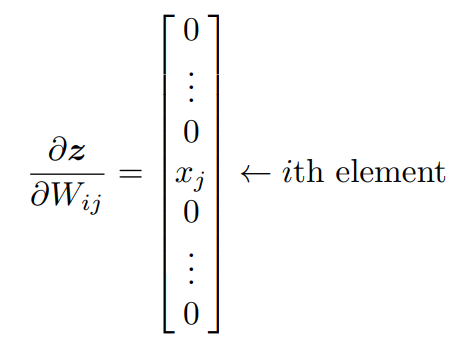
\includegraphics[scale=0.3]{img/softmax_deriv.png}
    \end{center}
    Now computing 
    \begin{equation}
      \frac{\partial L}{\partial W_{ij}} = \frac{\partial L}{\partial \mathbf{z}} \frac{\partial \mathbf{z}}{\partial W_{ij}} = (\mathbf{a} - \mathbf{y}) \frac{\partial \mathbf{z}}{\partial W_{ij}} = \sum_{k=1}^K (a_k - y_k) \frac{\partial z_k}{\partial W_{ij}} = (a_i - y_i) x_j
    \end{equation}
    To get $\partial L / \partial W_{ij}$ we want a matrix whose entry $(i, j)$ is $(a_i - y_i) x_j$. This is simply the outer product as shown below. For the bias term, $\partial \mathbf{z} / \partial \mathbf{b}$ is simply the identity matrix. 
    \begin{equation}
      \frac{\partial L}{\partial \mathbf{W}} = (\mathbf{a} - \mathbf{y}) \mathbf{x}^T, \;\;\;\; \frac{\partial L}{\partial \mathbf{b}} = \mathbf{a} - \mathbf{y}
    \end{equation}

    Therefore, summing the gradient over some minibatch $M \subset [N]$ gives 
    \begin{equation}
      \nabla_{\mathbf{W}} \ell_M = \sum_{i \in M} (\mathbf{h}_{\boldsymbol{\theta}}(\mathbf{x}^{(i)}) - \mathbf{y}^{(i)}) (\mathbf{x}^{(i)})^T, \;\;\;\;\; \nabla_{\mathbf{b}} \ell_M = \sum_{i \in M} (\mathbf{h}_{\boldsymbol{\theta}}(\mathbf{x}^{(i)}) - \mathbf{y}^{(i)})
    \end{equation}
    and our stochastic gradient descent algorithm is 
    \begin{align*}
      \boldsymbol{\theta} = \begin{pmatrix} \mathbf{W} \\ \mathbf{b} \end{pmatrix} & = \begin{pmatrix} \mathbf{W} \\ \mathbf{b} \end{pmatrix} - \eta \begin{pmatrix} \nabla_{\mathbf{W}} \ell_M \\ \nabla_{\mathbf{b}} \ell_M \end{pmatrix} \\
      & = \begin{pmatrix} \mathbf{W} \\ \mathbf{b} \end{pmatrix} - \eta \begin{pmatrix} \sum_{i \in M} (\mathbf{h}_{\boldsymbol{\theta}}(\mathbf{x}^{(i)}) - \mathbf{y}^{(i)}) (\mathbf{x}^{(i)})^T \\ \sum_{i \in M} (\mathbf{h}_{\boldsymbol{\theta}}(\mathbf{x}^{(i)}) - \mathbf{y}^{(i)}) \end{pmatrix} 
    \end{align*}
  \end{theorem}

